\begin{enumerate}
	\item Exercício
	
	\begin{figure}[H]
		\centering
		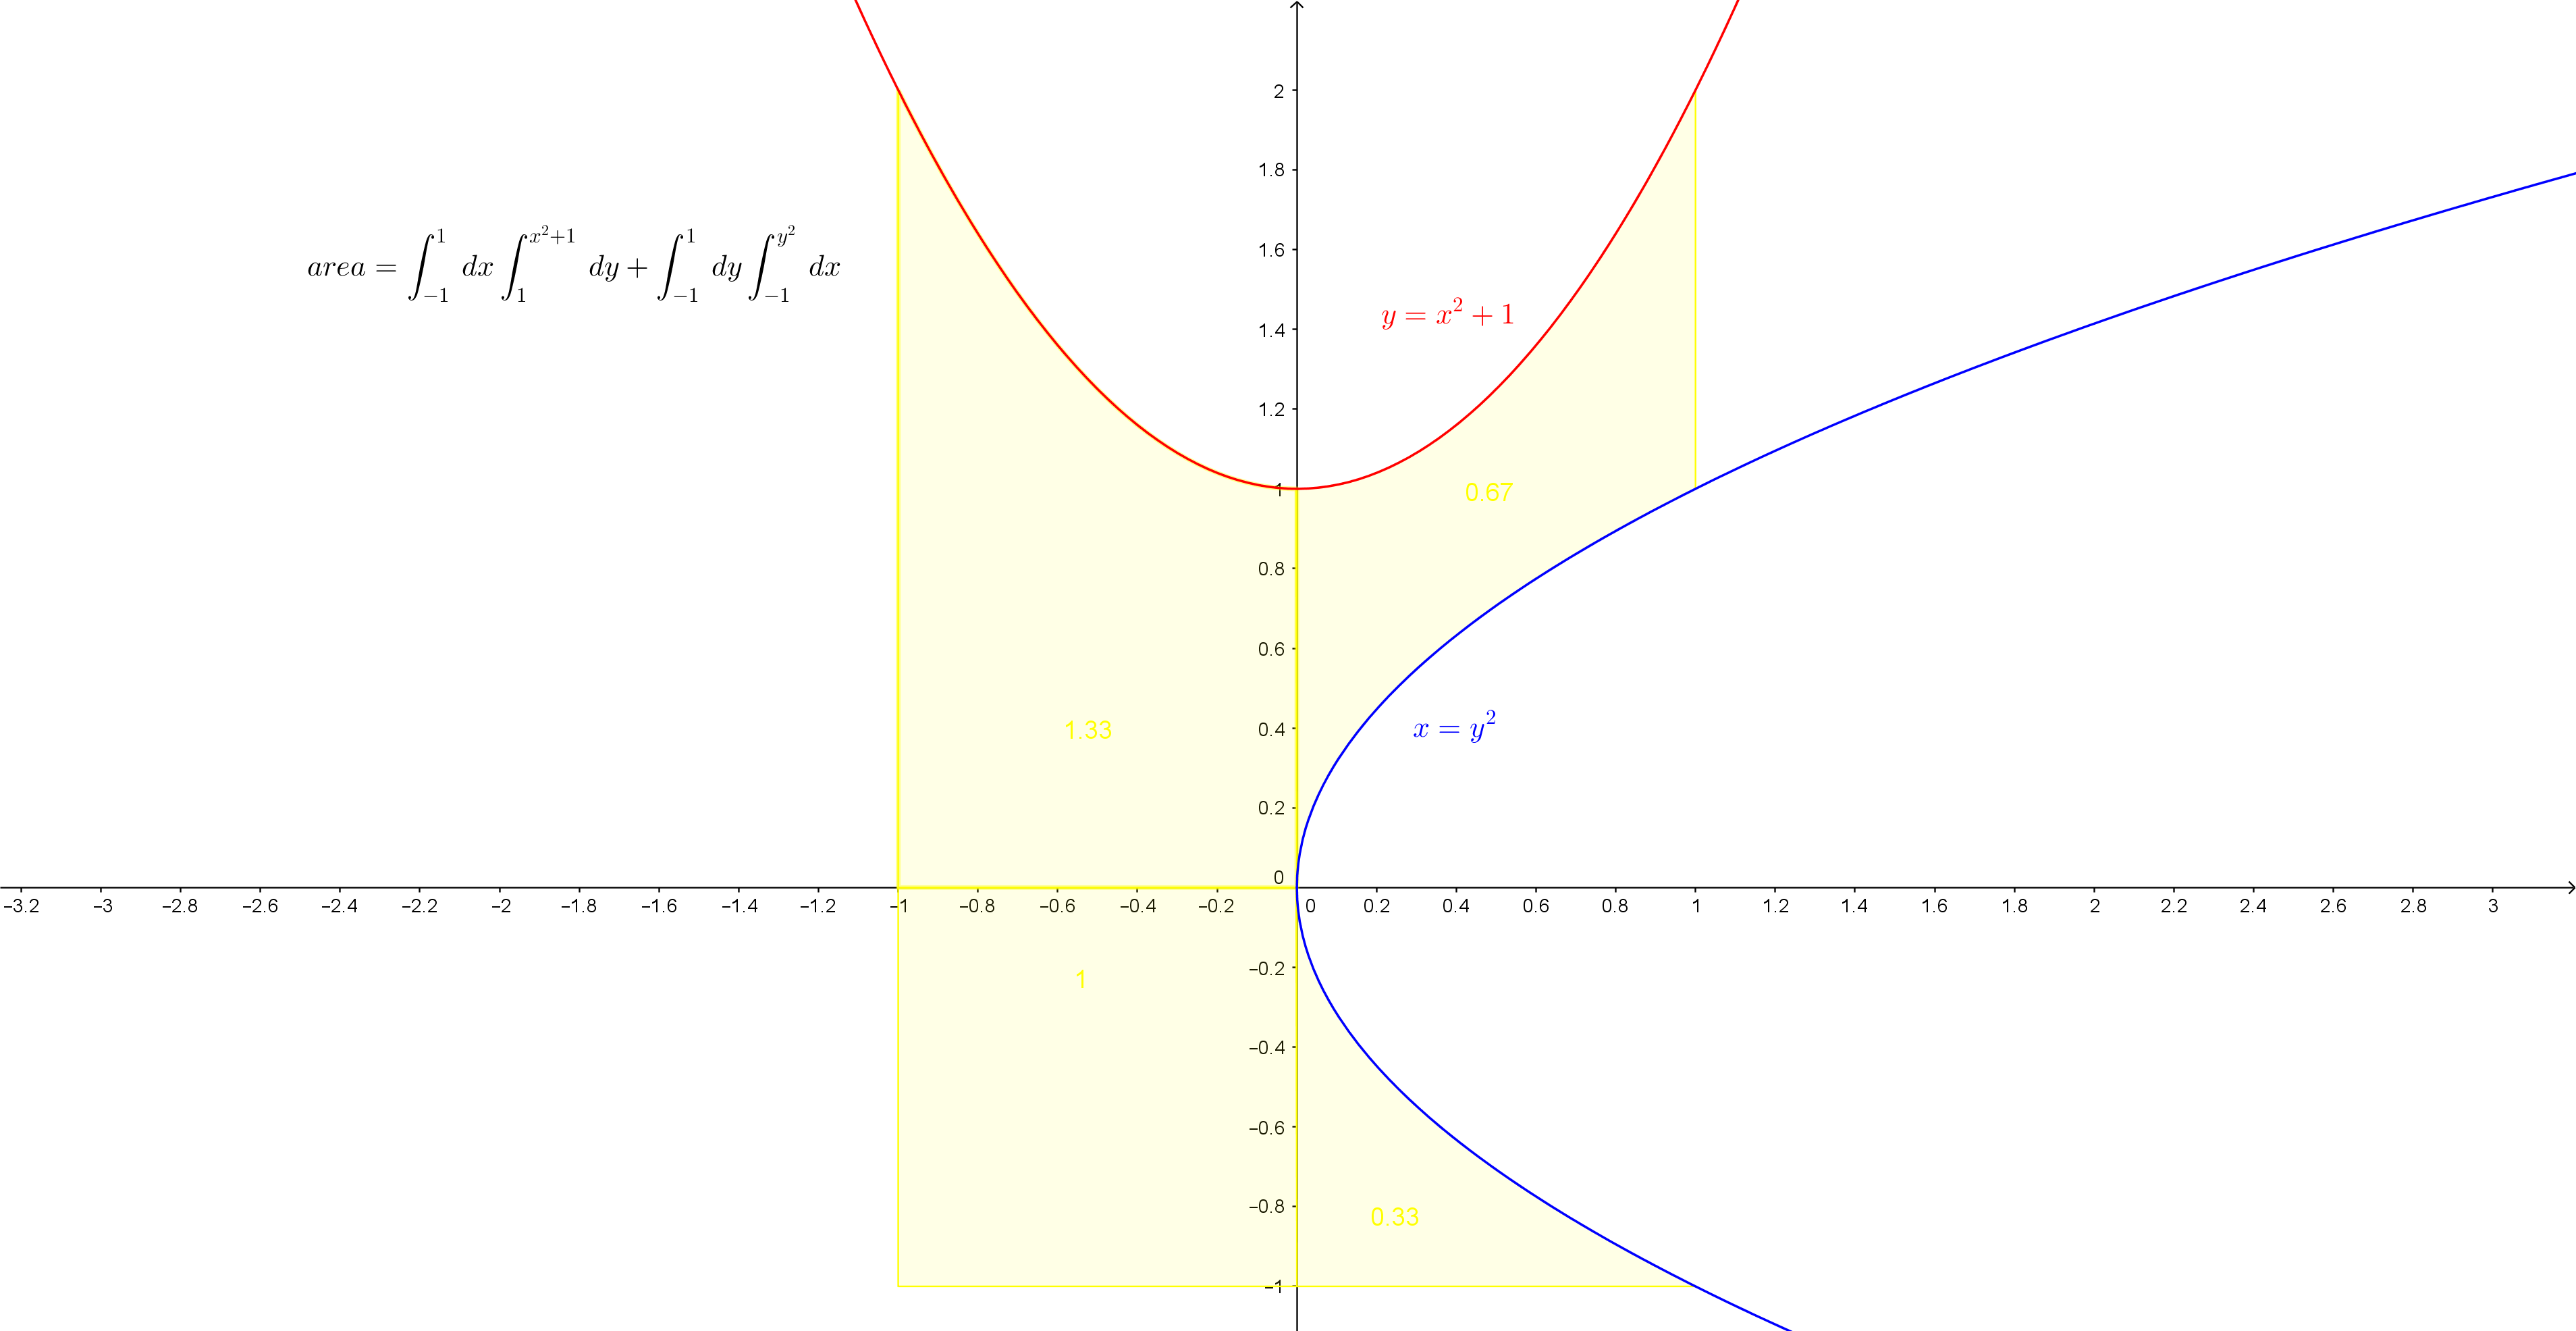
\includegraphics[width=\textwidth]{v08_a08_e01.png}
		\caption{Integrais duplas - Aula 8 - Exercício I}
		\label{v08_a08_e01}
	\end{figure}
	
	$a = \integral_{-1}^0 dx \integral_0^{x^2 + 1} dy + \integral_{-1}^0 dx \integral_{-1}^0 dy + \integral_0^{y^2} dx \integral_{-1}^0 dy + \integral_0^1 dx \integral_{\sqrt{x}}^{x^2 + 1} =\\ \integral_{-1}^0 dx\left(\integral_0^{x^2 + 1} dy + \integral_{-1}^0 dy\right)  + \integral_0^{y^2} dx \integral_{-1}^0 dy + \integral_0^1 dx \integral_{\sqrt{x}}^{x^2 + 1} = \integral_{-1}^0 dx \left([y]_0^{x^2 + 1} + [y]_{-1}^0\right)  + \integral_{-1}^0 dy\, [x]_0^{y^2} + \integral_0^1 dx\, [y]_{\sqrt{x}}^{x^2 + 1} = \integral_{-1}^0 dx\, \left(x^2 + 1 + 1\right) + \integral_{-1}^0 dy\, y^2 + \integral_0^1 dx\, \left(x^2 + 1 - \sqrt{x}\right) = \integral_{-1}^0 \left(x^2 + 2\right) dx + \integral_{-1}^0 y^2\, dy + \integral_0^1 \left(x^2 - x^{\frac{1}{2}} + 1\right) dx = \left[\dfrac{x^3}{3} + 2x\right]_{-1}^0 + \left[\dfrac{y^3}{3}\right]_{-1}^0 + \left[\dfrac{x^3}{3} - \dfrac{x^{\frac{3}{2}}}{\left(\dfrac{3}{2}\right)} + x\right]_0^1 = \left[\dfrac{x^3 + 6x}{3}\right]_{-1}^0 + \dfrac{1}{3}\left[y^3\right]_{-1}^0 + \left[\dfrac{x^3}{3} - \dfrac{2\sqrt{x^3}}{3} + x\right]_0^1 = \dfrac{1}{3}\left[x\left(x^2 + 6\right)\right]_{-1}^0 + \dfrac{1}{3}\left[\overstrike{0^3} - (-1)^3\right] + \left[\dfrac{x^3 - 2\sqrt{x^3} + 3x}{3}\right]_0^1 =\\ \dfrac{1}{3}\left[\overstrike{0\left(0^2 + 6\right)} - (-1)\left((-1)^2 + 6\right)\right] + \dfrac{1}{3} + \dfrac{1}{3}\left[x^3 - 2\sqrt{x^3} + 3x\right]_0^1 = \dfrac{7}{3} + \dfrac{1}{3} + \dfrac{1}{3}\left[1^3 - 2\sqrt{1^3} + 3\cdot1 \overstrike{- \left(0^3 - 2\sqrt{0^3} + 3\cdot0\right)}\right] = \dfrac{7}{3} + \dfrac{1}{3} + \dfrac{2}{3} = \dfrac{7 + 1 + 2}{3} = \dfrac{10}{3} = 3,\overline{3}$\newline\newline
	$a = \integral_{-1}^1 dx \integral_1^{x^2 + 1} dy + \integral_{-1}^{y^2} dx \integral_{-1}^1 dy = \integral_{-1}^1 dx\, [y]_1^{x^2 + 1} + \integral_{-1}^1 dy\, [x]_{-1}^{y^2} = \integral_{-1}^1 dx\, \left(x^2 \overstrike{+ 1 - 1}\right) + \integral_{-1}^1 dy\, \left(y^2 + 1\right) = \left[\dfrac{x^3}{3}\right]_{-1}^1 + \left[\dfrac{y^3}{3} + y\right]_{-1}^1 = \dfrac{1}{3}\left[x^3\right]_{-1}^1 + \dfrac{1}{3}\left[y\left(y^2 + 3\right)\right]_{-1}^1 = \dfrac{1}{3}\left(\left[1^3 - (-1)^3\right] + \left[1\left(1^2 + 3\right) - (-1)\left((-1)^2 + 3\right)\right]\right)\dfrac{1}{3}(2 + 4 + 4) = \frac{10}{3} = 3,\overline{3}$
\end{enumerate}